\documentclass[report/main.tex]{subfiles}

% A description and illustration of:

% - How do you interact as developers?
% - How is the team organized?
% - A complete description of stages and tools included in the CI/CD chains.
%     - That is, including deployment and release of your systems.
% - Organization of your repositor(ies).
%     - That is, either the structure of of mono-repository or organization of artifacts across repositories.
%     - In essence, it has to be be clear what is stored where and why.
% - Applied branching strategy.
% - Applied development process and tools supporting it
%     - For example, how did you use issues, Kanban boards, etc. to organize open tasks
% - How do you monitor your systems and what precisely do you monitor?
% - What do you log in your systems and how do you aggregate logs?
% - Brief results of the security assessment.
% - Applied strategy for scaling and load balancing.

% In essence it has to be clear how code or other artifacts come from idea into the running system and everything that happens on the way.

\begin{document}
    \section{Process' Perspective}
    \label{Sec:process_perspective}
        Some more text
        
        \subsection{Development Strategy}
            TODO: fancy intro here
            
            \subsubsection{Tools used}
                The teams aimed at doing agile development via including practices like self organising teams and iterative delivery (TODO). This becomes more once the teams Kanban board is explained
            
                For communication between the team members a Teams Group was used, which contained a general chat, a chat for arranging meetings and a chat that contains various useful links
                
                To host the code a Github Repository was used, which was owned by one group member
                
                Github Actions
                
                Github Projects
                
                Digital Ocean Droplet
                
                Digital Ocean Database Cluster
                
            
        \subsection{Monitoring}
            \subsubsection{Setup}
                The monitoring of the EvilTwitter application was done using the monitoring and alerting toolkit Prometheus\footnote{\hyperlink{https://prometheus.io/}{https://prometheus.io/}} to gather information from the application. Two dotnet package was used to retrieve data from the application. Prometheus-net.SystemMetrics\footnote{\hyperlink{https://github.com/Daniel15/prometheus-net.SystemMetrics}{https://github.com/Daniel15/prometheus-net.SystemMetrics}} was used to retreive system information from where the application was running, and prometheus-net\footnote{\hyperlink{https://github.com/prometheus-net/prometheus-net}{https://github.com/prometheus-net/prometheus-net}} to gather information from the Controllers
                
                Grafana\footnote{\hyperlink{https://grafana.com/}{https://grafana.com/}} was used to interpret this data and gain valuable information
            
            \subsubsection{TODO: title}
                The information gathered in Grafana was setup in 3 categories: 1. Alerts, 2. Controller usage, 3. System.
                
                % TODO: maybe two figures?!?!?
                \begin{figure}[H]
                    \centering
                    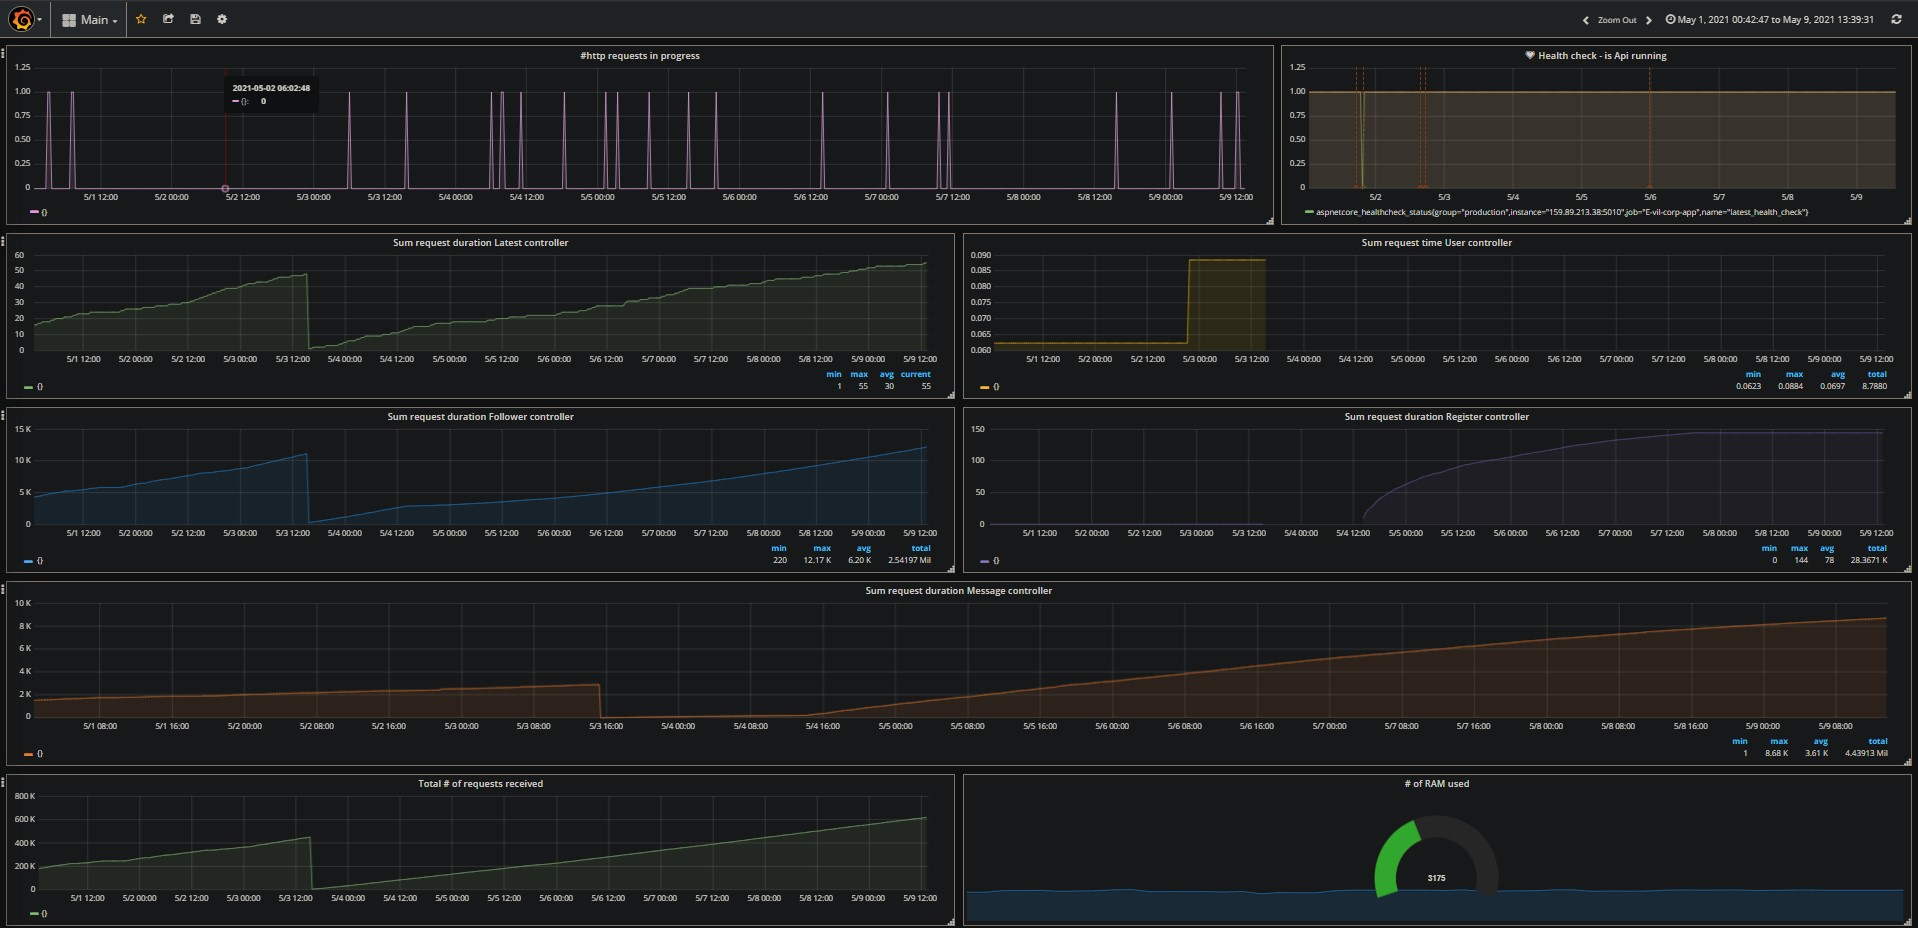
\includegraphics[width=\textwidth]{report/images/Grafana Setup.jpg}
                    \caption{Caption}
                    \label{fig:grafana_setup}
                \end{figure}
            
                First the alert graph can be seen at the top right, which is a value that can be either 1 or 0. This translates to what value latest returned last, with any latest value greater than 0 would resolved to a value of 1 and anything else would resolved to a value of 0. Hence if the Api is down or returns odd values this would be registered by Grafana
            
        \subsection{Logging}
        %Lukas
        
        \subsection{Security assessment}
            
\end{document}